\documentclass{article}%
\usepackage[T1]{fontenc}%
\usepackage[utf8]{inputenc}%
\usepackage{lmodern}%
\usepackage{textcomp}%
\usepackage{lastpage}%
\usepackage{parskip}%
\usepackage[top=4cm,hmargin=2cm,headheight=65pt,footskip=65pt]{geometry}%
\usepackage{amsmath}%
\usepackage{graphicx}%
\usepackage{needspace}%
\usepackage{color}%
\usepackage{longtable}%
\usepackage{multirow}%
\usepackage[table]{xcolor}%
\usepackage{fancyhdr}%
\usepackage{tabularx}%
%
\definecolor{OsdagGreen}{HTML}{D5DF93}%
\fancypagestyle{header}{ 
\renewcommand{\headrulewidth}{0pt}%
\renewcommand{\footrulewidth}{0pt}%
\fancyhead{ 
}%
\fancyfoot{ 
}%
\fancyhead[C]{ 
\begin{tabularx}{\textwidth}{|l|p{6cm}|l|X|}%
\hline%
\rowcolor{OsdagGreen}%
Company Name&&Project Title&\\%
\hline%
\rowcolor{OsdagGreen}%
Group/Team Name&&Subtitle&\\%
\hline%
\rowcolor{OsdagGreen}%
Designer&&Job Number&\\%
\hline%
\rowcolor{OsdagGreen}%
Date&10 /06 /2020&Client&\\%
\hline%
\end{tabularx}
}%
\fancyfoot[R]{ 
Page \thepage
}
}%
%
\begin{document}%
\normalsize%
\fontsize{8}{12}%
\selectfont%
\pagestyle{header}%
\section{Input Parameters}%
\label{sec:InputParameters}%
\renewcommand{\arraystretch}{1.2}%
\begin{longtable}{|p{5cm}|p{2cm}|p{2cm}|p{2cm}|p{5cm}|}%
\hline%
\hline%
\multicolumn{3}{|c|}{Module}&\multicolumn{2}{|c|}{Tension Members Welded Design}\\%
\hline%
\hline%
\multicolumn{3}{|c|}{Axial (kN)}&\multicolumn{2}{|c|}{500.0}\\%
\hline%
\hline%
\multicolumn{3}{|c|}{Length (mm) *}&\multicolumn{2}{|c|}{5000.0}\\%
\hline%
\hline%
\multicolumn{3}{|c|}{Section Size*}&\multicolumn{2}{|c|}{Ref List of Input Section}\\%
\hline%
\hline%
\multicolumn{5}{|c|}{\textbf{Plate Details}}\\%
\hline%
\multicolumn{3}{|c|}{\multirow{5}{*}{Plate Thickness (mm)*}}&\multicolumn{2}{|c|}{{[}3.0, 4.0, 6.0, 8.0, 10.0, 12.0}\\%
\multicolumn{3}{|c|}{\multirow{5}{*}{}}&\multicolumn{2}{|c|}{, 14.0, 16.0, 20.0, 22.0, 24.0}\\%
\multicolumn{3}{|c|}{\multirow{5}{*}{}}&\multicolumn{2}{|c|}{, 25.0, 26.0, 28.0, 30.0, 32.0}\\%
\multicolumn{3}{|c|}{\multirow{5}{*}{}}&\multicolumn{2}{|c|}{, 36.0, 40.0, 45.0, 50.0, 56.0}\\%
\multicolumn{3}{|c|}{\multirow{5}{*}{}}&\multicolumn{2}{|c|}{, 63.0, 80.0{]}}\\%
\hline%
\hline%
\multicolumn{3}{|c|}{Material}&\multicolumn{2}{|c|}{E 250 (Fe 410 W)B}\\%
\hline%
\hline%
\multicolumn{3}{|c|}{Ultimate strength, fu (MPa)}&\multicolumn{2}{|c|}{410}\\%
\hline%
\hline%
\multicolumn{3}{|c|}{Yield Strength , fy (MPa)}&\multicolumn{2}{|c|}{250}\\%
\hline%
\hline%
\multicolumn{5}{|c|}{\textbf{Weld Details}}\\%
\hline%
\hline%
\multicolumn{3}{|c|}{Weld Type}&\multicolumn{2}{|c|}{Fillet}\\%
\hline%
\hline%
\multicolumn{3}{|c|}{Type of weld fabrication}&\multicolumn{2}{|c|}{Shop Weld}\\%
\hline%
\hline%
\multicolumn{3}{|c|}{Material grade overwrite (MPa) Fu}&\multicolumn{2}{|c|}{410.0}\\%
\hline%
\hline%
\multicolumn{5}{|c|}{\textbf{Safety Factors {-} IS 800:2007 Table 5 (Clause 5.4.1) }}\\%
\hline%
\hline%
\multicolumn{3}{|c|}{Governed by Yielding}&\multicolumn{2}{|c|}{$\begin{aligned}\gamma_{m0}&=1.1\end{aligned}$}\\%
\hline%
\hline%
\multicolumn{3}{|c|}{Governed by Ultimate Stress}&\multicolumn{2}{|c|}{$\begin{aligned}\gamma_{m1}&=1.25\end{aligned}$}\\%
\hline%
\hline%
\multicolumn{3}{|c|}{Connection Weld}&\multicolumn{2}{|c|}{$\begin{aligned}\gamma_{mw}&=1.25\end{aligned}$}\\%
\hline%
\end{longtable}%
\subsection{List of Input Section}%
\label{subsec:ListofInputSection}%
\renewcommand{\arraystretch}{1.2}%
\begin{longtable}{|p{8cm}|p{8cm}|}%
\hline%
\multicolumn{1}{|c|}{Section Size*}&\multicolumn{1}{|c|}{{[}'MC 75', 'MC 100', 'MC 125', 'MC 125*', 'MC 150', 'MC 150*', 'MC 175', 'MC 175*', '}\\%
\hline%
\hline%
\multicolumn{1}{|c|}{ }&\multicolumn{1}{|c|}{MC 200', 'MC 200*', 'MC 225', 'MC 225*', 'MC 250', 'MC 250*', 'MC 250*', 'MC 300', }\\%
\hline%
\hline%
\multicolumn{1}{|c|}{ }&\multicolumn{1}{|c|}{'MC 300*', 'MC 300*', 'MC 350', 'MC 400', 'JC 100', 'JC 125', 'JC 150', 'JC 175', '}\\%
\hline%
\hline%
\multicolumn{1}{|c|}{ }&\multicolumn{1}{|c|}{JC 200', 'LC 75', 'LC 100', 'LC 125', 'LC (P) 125', 'LC 150', 'LC (P) 150', 'LC 175}\\%
\hline%
\hline%
\multicolumn{1}{|c|}{ }&\multicolumn{1}{|c|}{', 'LC 200', 'LC (P) 200', 'LC 225', 'LC 250', 'LC 300', 'LC (P) 300', 'LC 350', 'L}\\%
\hline%
\hline%
\multicolumn{1}{|c|}{ }&\multicolumn{1}{|c|}{C 400', 'MPC 75', 'MPC 100', 'MPC 125', 'MPC 125*', 'MPC 150', 'MPC 150*', 'MPC 175}\\%
\hline%
\hline%
\multicolumn{1}{|c|}{ }&\multicolumn{1}{|c|}{', 'MPC 175*', 'MPC 200', 'MPC 200*', 'MPC 225', 'MPC 225*', 'MPC 250', 'MPC 250*',}\\%
\hline%
\hline%
\multicolumn{1}{|c|}{ }&\multicolumn{1}{|c|}{ 'MPC 250*', 'MPC 300', 'MPC 300*', 'MPC 300*', 'MPC 350', 'MPC 400'{]}}\\%
\hline%
\end{longtable}

%
\Needspace{10\baselineskip}%
\section{Design Checks}%
\label{sec:DesignChecks}%
\subsection{Selected Member Data}%
\label{subsec:SelectedMemberData}%
\renewcommand{\arraystretch}{1.2}%
\begin{longtable}{|p{5cm}|p{2cm}|p{2cm}|p{2cm}|p{5cm}|}%
\hline%
\hline%
\multirow{13}{*}{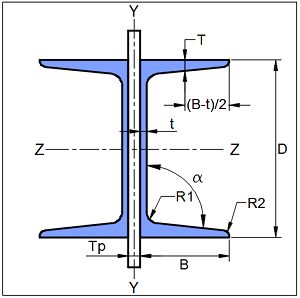
\includegraphics[width=5cm,height=5cm]{E:/workspace/Osdag3/ResourceFiles/images/Slope_BBChannel.png}}&\multicolumn{2}{|c|}{Section Size*}&\multicolumn{2}{|c|}{('MC 100', 'Back to Back Channels')}\\%
\cline{2%
-%
5}%
&\multicolumn{2}{|c|}{Material}&\multicolumn{2}{|c|}{E 250 (Fe 410 W)B}\\%
\cline{2%
-%
5}%
&\multicolumn{2}{|c|}{Ultimate strength, fu (MPa)}&\multicolumn{2}{|c|}{410}\\%
\cline{2%
-%
5}%
&\multicolumn{2}{|c|}{Yield Strength , fy (MPa)}&\multicolumn{2}{|c|}{250}\\%
\cline{2%
-%
5}%
&Mass&9.56&Iz(mm4)&3820000.0\\%
\cline{2%
-%
5}%
&Area(mm2) {-} A&1210.0&Iy(mm4)&1099900.0\\%
\cline{2%
-%
5}%
&D(mm)&100&rz(mm)&39.7\\%
\cline{2%
-%
5}%
&B(mm)&50&ry(mm)&21.3\\%
\cline{2%
-%
5}%
&t(mm)&5.0&Zz(mm3)&76400.0\\%
\cline{2%
-%
5}%
&T(mm)&7.7&Zy(mm3)&22000.0\\%
\cline{2%
-%
5}%
&FlangeSlope&96&Zpz(mm3)&88960.0\\%
\cline{2%
-%
5}%
&R1(mm)&9.0&Zpy(mm3)&414340.0\\%
\cline{2%
-%
5}%
&R2(mm)&2.4&r(mm)&21.32\\%
\cline{2%
-%
5}%
\hline%
\end{longtable}

%
\newpage%
\subsection{Member Checks}%
\label{subsec:MemberChecks}%
\renewcommand{\arraystretch}{1.2}%
\begin{longtable}{|p{2.5cm}|p{4.5cm}|p{8cm}|p{1cm}|}%
\hline%
\rowcolor{OsdagGreen}%
Check&Required&Provided&Remarks\\%
\hline%
\endhead%
\hline%
Tension Yielding Capacity (kN)&&$\begin{aligned}T_{dg}~or~A_c&= \frac{2 * A_g ~ f_y}{\gamma_{m0}}\\ &= \frac{2*1210.0*250}{1.1}\\ &= 550.0\end{aligned}$&\\%
\hline%
Tension Rupture Capacity (kN)&&$\begin{aligned}\beta &= 1.4 - 0.076*\frac{w}{t}*\frac{f_{y}}{0.9*f_{u}}*\frac{b_s}{L_c}\\ &\leq\frac{0.9*f_{u}*\gamma_{m0}}{f_{y}*\gamma_{m1}} \geq 0.7 \\ &= 1.4 - 0.076*\frac{50}{5.0}*\frac{250}{0.9*410}*\frac{50}{159 }\\ &\leq\frac{0.9* 410*1.1}{250*1.25} \geq 0.7 \\ &= 1.24\\ T_{dn} &= 2*(\frac{0.9*A_{nc}*f_{u}}{\gamma_{m1}} + \frac{\beta * A_{go} * f_{y}}{\gamma_{m0}})\\ &= 2*(\frac{0.9* 423.0*410}{1.25} + \frac{1.24*770.0*250}{1.1})\\ &= 683.74\end{aligned}$&\\%
\hline%
Tension Capacity (kN)&500.0&$\begin{aligned} T_d &= min(T_{dg},T_{dn})\\ &= min(550.0,683.74)\\ &=550.0\end{aligned}$&Pass\\%
\hline%
Slenderness&$\begin{aligned}\frac{K * L}{r} &\leq 400\end{aligned}$&$\begin{aligned}\frac{K * L}{r} &= \frac{1*5000.0}{21.32}\\ &= 234.53\end{aligned}$&Pass\\%
\hline%
Utilization Ratio&$\begin{aligned} Utilization~Ratio &\leq 1 \end{aligned}$&$\begin{aligned} Utilization~Ratio &= \frac{F}{Td}&=\frac{500.0}{550.0}\\ &= 0.91\end{aligned}$&\\%
\hline%
Axial Load Considered (kN)&$\begin{aligned} Ac_{min} &= 0.3 * A_c\\ &= 0.3 *550.0\\ &=165.0\\ Ac_{max} &=550.0\end{aligned}$&$\begin{aligned} A &=500.0\end{aligned}$&Pass\\%
\hline%
\end{longtable}

%
\newpage%
\subsection{Thickness Checks}%
\label{subsec:ThicknessChecks}%
\renewcommand{\arraystretch}{1.2}%
\begin{longtable}{|p{2.5cm}|p{5cm}|p{7.5cm}|p{1cm}|}%
\hline%
\rowcolor{OsdagGreen}%
Check&Required&Provided&Remarks\\%
\hline%
\endhead%
\hline%
Tension Yielding Capacity (kN)&500.0&$\begin{aligned} T_{dg} &= \frac{l*t*f_y}{\gamma_{mo}}\\ &=\frac{1*400*24.0*250}{1.1}\\ &=545.45\end{aligned}$&Pass\\%
\hline%
\end{longtable}

%
\newpage%
\subsection{Weld Checks}%
\label{subsec:WeldChecks}%
\renewcommand{\arraystretch}{1.2}%
\begin{longtable}{|p{3cm}|p{7cm}|p{5cm}|p{1cm}|}%
\hline%
\rowcolor{OsdagGreen}%
Check&Required&Provided&Remarks\\%
\hline%
\endhead%
\hline%
Min Weld Size (mm)&$\begin{aligned} & t_{w_{min}}~based~on~thinner~part\\ & =5~or~3\\ & IS800:2007~cl.10.5.2.3~Table 21\\ & t_{w_{min}}~based~on~thicker~part=6\end{aligned}$&5&Pass\\%
\hline%
Max Weld Size (mm)&$\begin{aligned} & Thickness~of~Thinner~part\\ &=min(24.0,5.0)=5.0\\ &t_{w_{max}} =5\end{aligned}$&5&Pass\\%
\hline%
Throat Thickness (mm)&$\begin{aligned} t_t &\geq 3 \end{aligned}$&$\begin{aligned} t_t & = 0.7* t_w \\ & = 0.7*5\\ t_t & = 3.5\end{aligned}$&Pass\\%
\hline%
Effective length (mm)&&$\begin{aligned} l_w &=756\end{aligned}$&\\%
\hline%
Weld Strength (kN/mm)&$\begin{aligned} R_w&=\sqrt{(T_{wh}+A_{wh})^2 + (T_{wv}+V_{wv})^2}\\ T_{wh}&=\frac{M*y_{max}}{I{pw}}=\frac{0.0*0.0}{1.0}\\ T_{wv}&=\frac{M*x_{max}}{I{pw}}=\frac{0.0*0.0}{1.0}\\ V_{wv}&=\frac{V}{l_w}=\frac{0.0}{756}\\ A_{wh}&=\frac{A}{l_w}=\frac{500000.0}{756}\\ R_w&=\sqrt{(0.0+661.38)^2 + (0.0+0.0)^2}\\ &=661.38\end{aligned}$&$\begin{aligned} f_w &=\frac{t_t*f_u}{\sqrt{3}*\gamma_{mw}}\\ &=\frac{3.5*410}{\sqrt{3}*1.25}\\ &=662.8\end{aligned}$&Pass\\%
\hline%
\end{longtable}

%
\newpage%
\subsection{Gusset Plate Checks}%
\label{subsec:GussetPlateChecks}%
\renewcommand{\arraystretch}{1.2}%
\begin{longtable}{|p{2.5cm}|p{5cm}|p{7.5cm}|p{1cm}|}%
\hline%
\rowcolor{OsdagGreen}%
Check&Required&Provided&Remarks\\%
\hline%
\endhead%
\hline%
Min.Height (mm)&&$\begin{aligned} H &= 1* Depth + clearance \\ &=(1*400)+30\\ &= 130\end{aligned}$&\\%
\hline%
Min.Length (mm)&5000.0&$\begin{aligned} L &= Flange weld + clearance \\ &= 144+30\\ &= 174\end{aligned}$&Pass\\%
\hline%
Thickness (mm)&&$\begin{aligned} t_p &=24.0\end{aligned}$&\\%
\hline%
Tension Yielding Capacity (kN)&&$\begin{aligned} T_{dg} &= \frac{l*t*f_y}{\gamma_{mo}}\\ &=\frac{1*400*24.0*250}{1.1}\\ &=545.45\end{aligned}$&\\%
\hline%
Tension Rupture Capacity (kN)&&$\begin{aligned} T_{dn} &= \frac{0.9*A_{n}*f_u}{\gamma_{m1}}\\ &=\frac{1*0.9*400*24.0*410}{1.25}\\ &=708.48\end{aligned}$&\\%
\hline%
Block Shear Capacity (kN)&&$\begin{aligned}T_{db1} &= \frac{A_{vg} f_{y}}{\sqrt{3} \gamma_{m0}} + \frac{0.9 A_{tn} f_{u}}{\gamma_{m1}}\\ T_{db2} &= \frac{0.9*A_{vn} f_{u}}{\sqrt{3} \gamma_{m1}} + \frac{A_{tg} f_{y}}{\gamma_{m0}}\\ T_{db} &= min(T_{db1}, T_{db2})= 1277.65\end{aligned}$&\\%
\hline%
Tension Capacity (kN)&$\begin{aligned} A &=500.0\end{aligned}$&$\begin{aligned} T_d &= min(T_{dg},T_{dn},T_{db})\\ &= min(545.45,708.48,1277.65)\\ &=545.45\end{aligned}$&Pass\\%
\hline%
\end{longtable}

%
\newpage%
\subsection{Intermittent Connection}%
\label{subsec:IntermittentConnection}%
\renewcommand{\arraystretch}{1.2}%
\begin{longtable}{|p{2.5cm}|p{5cm}|p{7.5cm}|p{1cm}|}%
\hline%
\rowcolor{OsdagGreen}%
Check&Required&Provided&Remarks\\%
\hline%
\endhead%
\hline%
Connection (nos)& &4&\\%
\hline%
Spacing (mm)&1000&930.4&Pass\\%
\hline%
Min.Height (mm)&&130&\\%
\hline%
Min.Length (mm)&&50&\\%
\hline%
\end{longtable}

%
\Needspace{10\baselineskip}%
\newpage%
\section{3D View}%
\label{sec:3DView}%


\begin{figure}[h!]%
\centering%
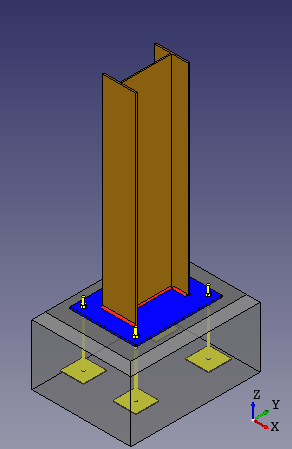
\includegraphics[width=\linewidth]{E:/workspace/Osdag3/ResourceFiles/images/3d.png}%
\caption{3D View}%
\end{figure}

%
\end{document}